% !TeX TXS-program:pdflatex = pdflatex -synctex=1 -interaction=nonstopmode --shell-escape %.tex
\documentclass[12pt]{report}
\usepackage[utf8]{inputenc}
%\usepackage[14pt]{extsizes}
\usepackage{listings}
\usepackage{indentfirst}
\usepackage{geometry}
\usepackage{textcomp}
\usepackage{amssymb}
\usepackage{amsmath}
\usepackage{amsthm} 
\usepackage{caption}
\usepackage{misccorr}
\usepackage[noadjust]{cite}
\usepackage{cmap} 
\usepackage[T2A]{fontenc}
\usepackage[english, russian]{babel}
\usepackage{graphics}
\usepackage{graphicx}
\usepackage{textcomp}
\usepackage{verbatim}
\usepackage{makeidx}
\usepackage{float}
\usepackage{bm}
\usepackage{esint}
\usepackage{mathtools}
\usepackage{graphicx}
\usepackage{listings}
% Для листинга кода:
\lstset{ %
language=python,                 % выбор языка для подсветки (здесь это С)
basicstyle=\small\sffamily, % размер и начертание шрифта для подсветки кода
numbers=left,               % где поставить нумерацию строк (слева\справа)
numberstyle=\tiny,           % размер шрифта для номеров строк
stepnumber=1,                   % размер шага между двумя номерами строк
numbersep=5pt,                % как далеко отстоят номера строк от подсвечиваемого кода
showspaces=false,            % показывать или нет пробелы специальными отступами
showstringspaces=false,      % показывать или нет пробелы в строках
showtabs=false,             % показывать или нет табуляцию в строках
frame=single,              % рисовать рамку вокруг кода
tabsize=2,                 % размер табуляции по умолчанию равен 2 пробелам
captionpos=t,              % позиция заголовка вверху [t] или внизу [b] 
breaklines=true,           % автоматически переносить строки (да\нет)
breakatwhitespace=false, % переносить строки только если есть пробел
escapeinside={\#*}{*)}   % если нужно добавить комментарии в коде
}


% plot
\usepackage{pgfplots}
\usepackage{filecontents}
\usetikzlibrary{datavisualization}
\usetikzlibrary{datavisualization.formats.functions}

% Для измененных титулов глав:
\usepackage{titlesec, blindtext, color} % подключаем нужные пакеты
\definecolor{gray75}{gray}{0.75} % определяем цвет
\newcommand{\hsp}{\hspace{20pt}} % длина линии в 20pt
% titleformat определяет стиль
\titleformat{\chapter}[hang]{\Huge\bfseries}{\thechapter\hsp\textcolor{gray75}{|}\hsp}{0pt}{\Huge\bfseries}

\makeatletter
\def\@biblabel#1{#1. }
\makeatother

\usepackage{hyperref}

\newcommand{\specchapter}[1]{\chapter*{#1}\addcontentsline{toc}{chapter}{#1}}
\newcommand{\specsection}[1]{\section*{#1}\addcontentsline{toc}{section}{#1}}
\newcommand{\specsubsection}[1]{\subsection*{#1}\addcontentsline{toc}{subsection}{#1}}

% геометрия
\geometry{pdftex, left = 2cm, right = 2cm, top = 2.5cm, bottom = 2.5cm}

\titlespacing{\chapter}{0pt}{-30pt}{20pt}

\setcounter{tocdepth}{4} % фикс переноса 
\righthyphenmin = 2
\tolerance = 2048

\begin{document}
%\def\chaptername{} % убирает "Глава"
\thispagestyle{empty}
\renewcommand\bibname{Список литературы}

\vspace{\baselineskip}
\noindent \begin{minipage}{0.15\textwidth}
	
\includegraphics[width=\linewidth]{bmstu}
\end{minipage}
\noindent\begin{minipage}{0.9\textwidth}
	\centering
	\textbf{Министерство науки и высшего образования Российской Федерации}\\
	\textbf{Федеральное государственное бюджетное образовательное учреждение высшего образования}\\
	\textbf{«Московский государственный технический университет имени Н.Э.~Баумана}\\
	\textbf{(национальный исследовательский университет)»}\\
	\textbf{(МГТУ им. Н.Э.~Баумана)}
\end{minipage}

\noindent\rule{18cm}{3pt}
\newline\newline
\noindent ФАКУЛЬТЕТ $\underline{\text{«Информатика и системы управления»}}$ \newline\newline
\noindent КАФЕДРА $\underline{\text{«Программное обеспечение ЭВМ и информационные технологии»}}$\newline\newline\newline\newline\newline\newline\newline


\begin{center}
\Large\textbf{Лабораторная работа № 2}
\end{center}
\vspace{\baselineskip}
\noindent\textbf{Дисциплина} $\underline{\text{Анализ алгоритмов~~~~~~~~~~~~~~~~~~~~~~~~~~~~~~~}}$\newline\newline
\noindent\textbf{Тема} $\underline{\text{Трудоемкость алгоритмов умножения матриц~~~~~~}}$\newline\newline
\noindent\textbf{Студент} $\underline{\text{Искакова К. М.~~~~~~~~~~~~~~~~~~~~~~~~~~~~~~~~~~~~~~~~~~~~~}}$\newline\newline
\noindent\textbf{Группа} $\underline{\text{ИУ7-52Б~~~~~~~~~~~~~~~~~~~~~~~~~~~~~~~~~~~~~~~~~~~~~~~~~~~~~~}}$\newline\newline
\noindent\textbf{Оценка (баллы)} $\underline{\text{~~~~~~~~~~~~~~~~~~~~~~~~~~~~~~~~~~~~~~~~~~~~~~~~~~~~~}}$\newline\newline
\noindent\textbf{Преподаватель} $\underline{\text{Волкова Л. Л.~~~~~~~~~~~~~~~~~~~~~~~~~~~~~~~~~~~}}$\newline

\begin{center}
	\vfill
	Москва~---~\the\year
	~г.
\end{center}
\clearpage

\tableofcontents

\newpage
\chapter*{Введение}
\addcontentsline{toc}{chapter}{Введение}
\textbf{Матрицей} A размера $[m*n]$ называется прямоугольная таблица
чисел, функций или алгебраических выражений, содержащая m строк и n столбцов. Числа m и n определяют размер матрицы \cite{mtrbook}. 

\textbf{Умножение матриц} — одна из основных операций над матрицами.
Матрица, получаемая в результате операции умножения, называется
произведением матриц. Операция умножения двух матриц выполнима только в
том случае, если число столбцов в первом сомножителе равно числу строк во
втором; в этом случае говорят, что матрицы согласованы. В частности,
умножение всегда выполнимо, если оба сомножителя — квадратные матрицы
одного и того же порядка. Таким образом, из существования произведения AB
вовсе не следует существование произведения BA.
Алгоритмы умножения матриц активно применяются во всех областях, применяющих
линейную алгебру. Примеры использования:
\begin{itemize}
	\item компьютерная графика;
	\item физика;
	\item экономика и так далее.
\end{itemize}
\vspace{\baselineskip}

\textbf{Цель работы:} оценить трудоемкость алгоритмов умножения матриц и получить практический навык оптимизации алгоритмов.\vspace{\baselineskip} 

\textbf{Задачи работы:}
\begin{enumerate}
  	\item изучить алгоритмы умножения матриц: стандартный и алгоритм Винограда; 
  	\item оптимизировать алгоритм Винограда; 
  	\item оценить трудоемкость классического алгоритма умножения матриц, стандартного и оптимизированного алгоритма Винограда;
  	\item реализовать данные алгоритмы умножения матриц на одном из языков программирования;  
  	\item сравнить алгоритмы умножения матриц.
\end{enumerate}


\chapter{Аналитическая часть}

В данном разделе будет рассмотрено описание умножения
матриц.

\section{Описание классического умножения матриц}
Пусть даны две прямоугольные матрицы А и В размерности m на n и n на k соответсвенно: 
\[ \begin{bmatrix}
	a_{1,1} & ... & a_{1,n} \\
	... & ... & ... \\
	a_{m,1} & ... & a_{m,n} \\
\end{bmatrix} \]\\

\[ \begin{bmatrix}
	b_{1,1} & ... & b_{1,k} \\
	... & ... & ... \\
	b_{n,1} & ... & b_{n,k} \\
\end{bmatrix} \]\\

В результате получим матрицу C размерности m на k:

\[ \begin{bmatrix}
	c_{1,1} & ... & c_{1,k} \\
	... & ... & ... \\
	c_{m,1} & ... & c_{m,k} \\
\end{bmatrix} \]\\


$c_{i,j} = \sum\limits_{l=1}^n a_{i,l}\cdot b_{l,j}$ называется произведением матриц A и B.

\section{Описание умножения матриц по Винограду}

Если посмотреть на результат умножения двух матриц, то видно, что каждый элемент в нем представляет собой скалярное произведение соответствующих строки и столбца исходных матриц. Можно заметить также, что такое умножение допускает предварительную обработку, позволяющую часть работы выполнить заранее.\vspace{\baselineskip}

Рассмотрим два вектора $V = (v1, v2, v3, v4)$ и $W = (w1, w2, w3, w4)$. Их скалярное произведение равно: 

$ V \cdot W=v_1 \cdot w_1 + v_2 \cdot w_2 + v_3 \cdot w_3 + v_4 \cdot w_4$ \\

Это равенство можно переписать в виде: \\
$V \cdot W=(v_1 + w_2) \cdot (v_2 + w_1) + (v_3 + w_4) \cdot (v_4 + w_3) - v_1 \cdot v_2 - v_3 \cdot v_4 - w_1 \cdot w_2 - w_3 \cdot w_4$\\

Менее очевидно, что выражение в правой части последнего равенства допускает предварительную обработку: его части можно вычислить заранее и запомнить для каждой строки первой матрицы и для каждого столбца второй. 
Это означает, что над предварительно обработанными элементами нам придется выполнять лишь первые два умножения и последующие пять сложений, а также дополнительно два сложения. 

В случае нечетной общей размерности происходит прибавление к каждому элементу матрицы произведения последнего элемента столбца первой матрицы на последний элемент строки второй матрицы



\chapter{Конструкторская часть}
В этом разделе содержатся cхемы алгоритмов умножения матриц.

\section{Оптимизации алгоритма умножения по Винограду}
В рамках данной лабораторной работы было предложено 3 оптимизации алгоритма умножения по Винограду:
\begin{enumerate}
	\item избавление от деления в условии цикла;
	\item замена $mulH[i] = mulH[i] + …$ на $mulH[i] += …$ (аналогично для других);
	\item накопление результата в буфер, чтобы не обращаться каждый раз к одной и той же ячейке памяти, и сброс буфера в ячейку матрицы после цикла.
\end{enumerate}
	
\section{Схемы алгоритмов}
На рис. 2.1-2.3 приведены схемы следующих алгоритмов:
\begin{enumerate}
	\item стандартный алгоритм умножения матриц;
	\item алгоритм умножения матриц по Винограду;
	\item оптимизированный алгоритм умножения матриц по Винограду;
\end{enumerate}

\newpage
\begin{figure}[h]
	\center{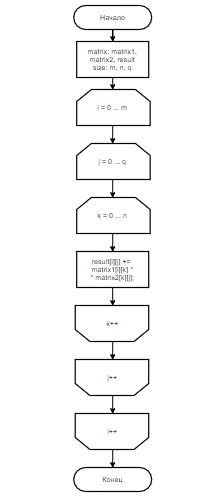
\includegraphics[scale=1]{standartSchema}}
	\caption{Стандартный алгоритм умножения матриц}
	\label{figure:image}
\end{figure}

\newpage
\begin{figure}[h]
	\center{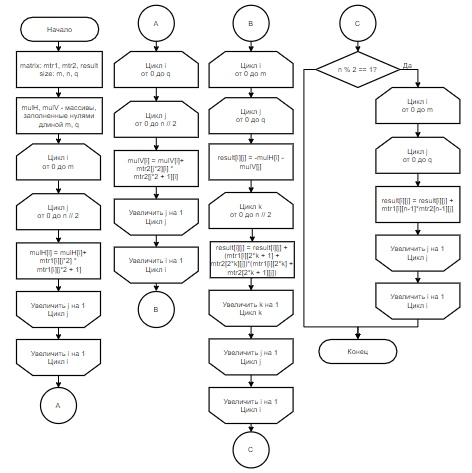
\includegraphics[scale=1]{vinogradSchema}}
	\caption{Алгоритм умножения матриц по Винограду}
	\label{figure:image}
\end{figure}

\newpage
\begin{figure}[h]
	\center{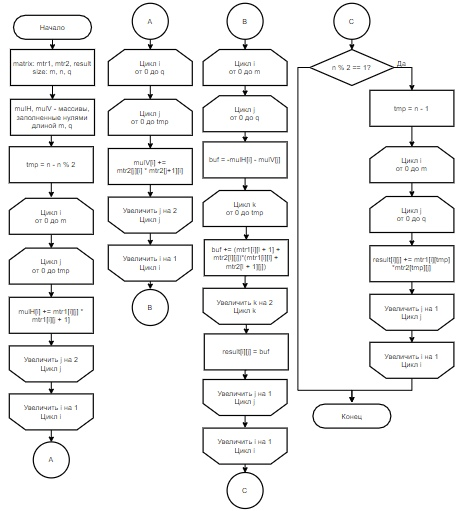
\includegraphics[scale=1]{vinogradOptSchema}}
	\caption{Оптимизированный алгоритм умножения матриц по Винограду}
	\label{figure:image}
\end{figure}



\chapter{Технологическая часть}
В данном разделе будут рассмотрены требования к программному обеспечению, средства реализации, представлен листинг кода, описание тестирования и трудоемкость алгоритмов.
\section{Требования к программному обеспечению}
\noindent\textbf{Требования к вводу:} на вход подаются две матрицы, размеры которых m x n и n x q соответственно.

\vspace{\baselineskip}
\noindent\textbf{Требования к программе:}
\begin{enumerate}
	\item на выходе
	необходимо получить матрицу, которая является результатом умножения двух матриц;
	\item требуется замерить время работы
	каждого из алгоритмов. 
\end{enumerate}
\section{Средства реализации}
В качестве языка программирования был выбран Python т.к. я знаком с данным языком, он простой и лаконичный, имеющий немногословный и понятный синтаксис, похожий на псевдокод, обладающий сильной динамической типизацией, которая способствует быстрому написанию кода. 

Среда разработки — PyCharm, которая предоставляет умную проверку кода, быстрое выявление ошибок и оперативное исправление, вкупе с автоматическим рефакторингом кода, и богатыми возможностями в навигации.  

Время  работы алгоритмов было замерено с помощью функции process\_time() из библиотеки time \cite{time}.

\newpage
\section{Листинг кода}

В листингах 3.1-3.3 представлена реализация алгоритмов умножения матриц.
\vspace{\baselineskip}

\begin{lstlisting}[label=some-code,caption=Стандартный алгоритм умножения матриц]
def classic(n, m, k, matr1, matr2, res):
	i = 0
	while i < n:
		j = 0
		while j < k:
			l = 0
			while l < m:
				res[i][j] += matr1[i][l] * matr2[l][j]
				l += 1
			j += 1
		i += 1
	return res
\end{lstlisting}

\begin{lstlisting}[label=some-code,caption=Алгоритм умножения матриц по Винограду]
def vinograd(n, m, k, matr1, matr2, res):
	mulH = [0] * n
	mulV = [0] * k
	
	i = 0
	while i < n:
		j = 0
		while j < m // 2:
			mulH[i] = mulH[i] + matr1[i][j * 2] * matr1[i][j * 2 + 1]
			j += 1
		i += 1
	
	i = 0
	while i < k:
		j = 0
		while j < m // 2:
			mulV[i] = mulV[i] + matr2[j * 2][i] * matr2[j * 2 + 1][i]
			j += 1
		i += 1
	
	i = 0
	while i < n:
		j = 0
		while j < k:
			res[i][j] = -mulH[i] - mulV[j]
			l = 0
			while l < m // 2:
				res[i][j] = res[i][j] + (matr1[i][2 * l + 1] + matr2[2 * l][j]) * \
										(matr1[i][2 * l] + matr2[2 * l + 1][j])
				l += 1
			j += 1
		i += 1
	
	if m % 2 == 1:
		i = 0
		while i < n:
			j = 0
			while j < k:
				res[i][j] = res[i][j] + matr1[i][m - 1] * matr2[m - 1][j]
				j += 1
			i += 1
	return res
\end{lstlisting}

\begin{lstlisting}[label=some-code,caption=Оптимизированный алгоритм умножения матриц по Винограду]
def vinograd_opt(n, m, k, matr1, matr2, res):
	mulH = [0] * n
	mulV = [0] * k
	
	tmp = m - m % 2
	
	i = 0
		while i < n:
			j = 0
			while j < tmp:
				mulH[i] += matr1[i][j] * matr1[i][j + 1]
				j += 2
			i += 1
	
	i = 0
	while i < k:
		j = 0
		while j < tmp:
			mulV[i] += matr2[j][i] * matr2[j + 1][i]
			j += 2
		i += 1
	
	i = 0
	while i < n:
		j = 0
		while j < k:
			buff = -mulH[i] - mulV[j]
			l = 0
			while l < tmp:
				buff += (matr1[i][l + 1] + matr2[l][j]) * (matr1[i][l] + matr2[l + 1][j])
				l += 2
			res[i][j] = buff
			j += 1
		i += 1
	
	if m % 2 == 1:
		i = 0
		tmp = m - 1
		while i < n:
			j = 0
			while j < k:
				res[i][j] += matr1[i][tmp] * matr2[tmp][j]
				j += 1
			i += 1
	return res
\end{lstlisting}

\newpage
\section{Трудоемкость алгоритмов}
Введем модель вычисления трудоемкости для оценки алгоритмов: 
\begin{itemize}
	\item базовые операции стоимостью 1: +, -, =, ==, <=, >=, !=, +=, -=, [];
	\item базовые операции стоимостью 2: *, /, \%, *=, /= ;
	\item оценка трудоемкости цикла: Fц = init +  N*(a + Fтела + post) + a, где a - условие цикла, init - предусловие цикла, post - постусловие цикла
	\item стоимость условного перехода применим за 0, стоимость вычисления условия остаётся
\end{itemize}

Оценим трудоемкость алгоритмов по коду программы.

\subsection{Трудоемкость стандартного алгоритма умножения матриц}
Рассмотрим трудоемкость стандартного алгоритма умножения матриц.\vspace{\baselineskip}

Подсчет: 2 + m * (2 + 2 + n * (2 + 2 + q * (2 + 6 + 2)))\vspace{\baselineskip}

Итог: 10*m*n*q + 4 * m * n + 4 * m + 2, где m, n, q – константы для матриц A с размерами m * n и B с размерами n * q 

\subsection{Трудоемкость алгоритма умножения матриц по Винограду}
Рассмотрим трудоемкость алгоритма умножения матриц по Винограду.\vspace{\baselineskip}

Инициализация mulH и mulV: 2 * 3\vspace{\baselineskip}

Заполнение mulH: 2 + m * (2 + 2 + n / 2 * (3 + 6 + 6))\vspace{\baselineskip}

Заполнение mulV: 2 + q * (2 + 2 + n / 2 * (3 + 6 + 6))\vspace{\baselineskip}

Подсчет результата: 2 + m * (2 + 2 + q * (2 + 7 + 2 + n / 2 * (3 + 23)))\vspace{\baselineskip}


Условие нечетности n: $\begin{bmatrix}
	2    &&, \text{невыполнение условия}\\
	2 + m *(2 + 2 + q * (2 + 8 + 5)) &&, \text{выполнение условия}\\
\end{bmatrix} $ \\
\vspace{\baselineskip}

Итог: 13 * m * n * q + 7.5 * m * n + 7.5 * n * q + 11 * m * q + 8 * m + 4 * q + 14 + + $\begin{bmatrix}
	2    \\
	15*m*q + 4*m + 2\\
\end{bmatrix} $, где m, n, q – константы для матриц A с размерами m * n и B с размерами n * q.

\subsection{Трудоемкость оптимизированного алгоритма умножения матриц по Винограду}
Рассмотрим трудоемкость оптимизированного алгоритма умножения матриц по Винограду.\vspace{\baselineskip}

Инициализация mulH и mulV: 2 * 3\vspace{\baselineskip}

Переменная tmp: 3\vspace{\baselineskip}

Заполнение mulH: 2 + m * (2 + 2 + n / 2 * (2 + 5 + 3))\vspace{\baselineskip}

Заполнение mulV: 2 + q * (2 + 2 + n / 2 * (2 + 5 + 3))\vspace{\baselineskip}ƒ

Подсчет результата: 2 + m * (2 + 2 + q * (2 + 5 + 3 + 2 + n / 2 * (2 + 14)))\vspace{\baselineskip}


Условие нечетности n: $\begin{bmatrix}
	2    &&, \text{невыполнение условия}\\
	2 + 2 + m * (2 + 2 + q * (2 + 6 + 2)) &&, \text{выполнение условия}\\
\end{bmatrix} $ \\
\vspace{\baselineskip}

Итог: 8 * m * n * q + 5 * m * n + 5 * n * q + 12 * m * q + 8 * m + 4 * q + 17 + + $\begin{bmatrix}
	2    \\
	10*m*q + 4*m + 2\\
\end{bmatrix} $, где m, n, q – константы для матриц A с размерами m * n и B с размерами n * q.

\newpage
\section{Тестирование}
Реализовано модульное тестирование отдельным файлом test.py с помощью библиотеки unittest \cite{unittest}. Полученные результаты функций сравниваются с контрольными значениями. \vspace{\baselineskip}

На  листингах 3.4-3.5 продемонстрированы функции, использованные для тесирования

\begin{lstlisting}[label=some-code,caption=Функция сравнения матриц]
def comp_matr(matr1, matr2):
	if len(matr1) != len(matr2):
		return False
	if len(matr1) == 0 or len(matr1[0]) != len(matr2[0]):
		return False
	for i in range(len(matr1)):
		for j in range(len(matr1[i])):
			if matr1[i][j] != matr2[i][j]:
				return False
	return True
\end{lstlisting}

\begin{lstlisting}[label=some-code,caption=Функция тестирования двух алгоритмов]
iteration = 10
for _ in range(iteration):
	size = [randint(1, iteration), randint(1, iteration), randint(1, iteration)]
	for _ in range(iteration):
		if not comp(size[0], size[1], size[2], func1, func2):
			err += 1
if err:
	print('Errors:  ', err)
else:
	print('Success')
\end{lstlisting}

\begin{flushleft}

\end{flushleft}

Программа успешно прошла все тестовые случаи, см. рис. 3.1. 

\begin{figure}[h]
	\center{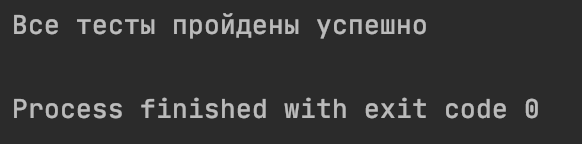
\includegraphics[scale=1]{testing}}
	\caption{Тестирование программы}
	\label{figure:image}
\end{figure}

\chapter{Экспериментальная часть}

В данном разделе приведены примеры работы программы и сравнительный анализ алгоритмов на основе экспериментальных данных. 

\section{Примеры работы} 
 
На рис. 4.1 представлено главное меню программы. 

\begin{figure}[h]
	\center{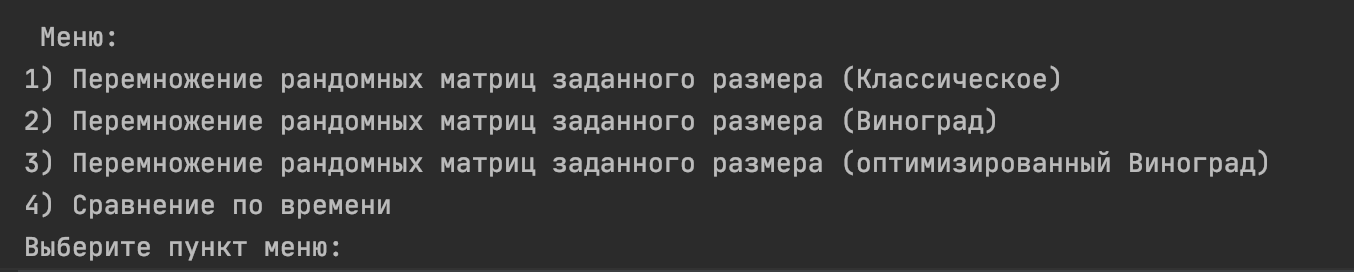
\includegraphics[scale=0.7]{menu}}
	\caption{Главное меню программы}
	\label{figure:image}
\end{figure}

На рис. 4.2-4.3 приведены примеры работы программы при выборе пункта меню 1.

\begin{figure}[h]
	\center{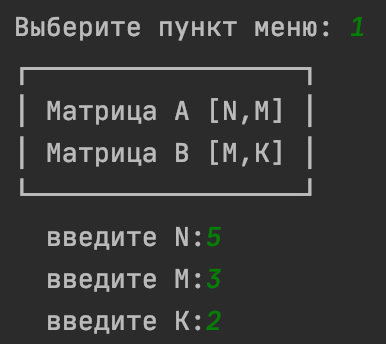
\includegraphics[scale=0.7]{choiceSt}}
	\caption{Выбор пункта меню 1 и ввод данных для создания матриц}
	\label{figure:image}
\end{figure}

\begin{figure}[h]
	\center{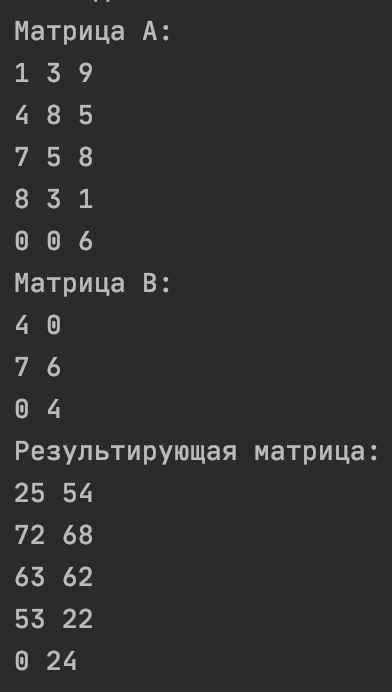
\includegraphics[scale=0.7]{resultMtr}}
	\caption{Полученный результат умножения}
	\label{figure:image}
\end{figure}

\newpage
На рис. 4.4 приведены примеры работы программы при выборе пункта меню 4.

\begin{figure}[h]
	\center{
\includegraphics[scale=0.7]{timeAnalyse}}
	\caption{Анализ по времени работы алгоритмов}
	\label{figure:image}
\end{figure}
 
\newpage
\section{Постановка эксперимента по замеру времени}

Для произведения замеров времени выполнения реализации алгоритмов будет использована формула: \begin{equation}\label{eq:fourierrow}
	t = \frac{T}{N}
\end{equation}
где t — среднее время выполнения алгоритма, N — количество замеров, T — время выполнения N замеров.  
Неоднократное измерение времени необходимо для получения более точного результа.  
 
 Количество замеров взято равным 100. Эксперимент проводится на квадратных матрицах, заполненных произвольными значениями.
 
 Был проведен замер времени работы каждого из алгоритмов, результат представлен в таблице 4.1. \vspace{\baselineskip}
 
\begin{table}[H]
	\caption{\label{tab:canonsummary}Сравнение алгоритмов по времени}
	\begin{center}
\begin{tabular}{ | l | l | l | }
	\hline
	Алгоритм умножения & Размер матриц & Время работы, сек \\ \hline
	Стандартный & 2 & 0.00001297 \\
	По Винограду & 2 & 0.00002456 \\
	По Винограду оптимизированный & 2 & 0.00001859 \\ \hline
	Стандартный & 3 & 0.00003906 \\
	По Винограду & 3 & 0.00005213 \\
	По Винограду оптимизированный & 3 & 0.00004844 \\ \hline
	Стандартный & 4 & 0.00009531 \\
	По Винограду & 4 & 0.00014245 \\
	По Винограду оптимизированный & 4 & 0.00010312 \\ \hline
	Стандартный & 5 & 0.00017656 \\
	По Винограду & 5 & 0.00022748 \\
	По Винограду оптимизированный & 5 & 0.00018906 \\ \hline
	Стандартный & 6 & 0.00030469 \\
	По Винограду & 6 & 0.00034123 \\
	По Винограду оптимизированный & 6 & 0.00030937 \\ \hline
	Стандартный & 7 & 0.00047813 \\
	По Винограду & 7 & 0.00054623 \\
	По Винограду оптимизированный & 7 & 0.00046406 \\ \hline
	Стандартный & 10 & 0.00136250 \\
	По Винограду & 10 & 0.00155625 \\
	По Винограду оптимизированный & 10 & 0.00119062 \\ \hline
	Стандартный & 25 & 0.02106250 \\
	По Винограду & 25 & 0.02340625 \\
	По Винограду оптимизированный & 25 & 0.01775000 \\ \hline
	Стандартный & 50 & 0.16750000 \\
	По Винограду & 50 & 0.17093750 \\
	По Винограду оптимизированный & 50 & 0.12218750 \\
	\hline
\end{tabular}
\end{center}
\end{table} 

\textbf{Вывод: } оптимизированный алгоритм умножения матриц по Винограду показывает наилучшее время на средних размерах, однако неоптимизированный алгоритм умножения матриц по Винограда показывает наихудшее время. Это связано с тем, что обычный алгоритм мало оптимизирован и приходится вычислять одни и те же значения несколько раз. Стандартный алгоритм умножения работает быстрее на малых размерах. Выбирать алгоритм необходимо в зависимости от поставленной задачи. Если требуется быстро перемножать  матрицы больших размеров, то оптимизированный алгоритм умножения матриц по Винограду справится с этой задачей быстрее. Если необходимо работать с матрицами малых размеров (< 7), то следует выбирать стандартный алгоритм умножения матриц.

\chapter*{Заключение}
\addcontentsline{toc}{chapter}{Заключение}

В ходе работы были изучены алгоритмы умножения матриц. Реализованы 3 алгоритма, приведен программный код реализации алгоритмов по умножению матриц.

Была подсчитана трудоемкость каждого из алгоритмов. А также было проведено сравнение алгоритмов по времени и трудоемкости.

Цель работы достигнута. Получены практические навыки реализации алгоритмов Винограда и стандартного алгоритма, а также проведена исследовательская работа по оптимизации и вычислении трудоемкости алгоритмов.


\begin{thebibliography}{2}
	\addcontentsline{toc}{chapter}{Список литературы}
	\bibitem{mtrbook} Курош А. Г. Курс высшей алгебры. — 9-е изд. — М.: Наука, 1968. — 432 с
	\bibitem{time} Официальный сайт Python, документация [электронный ресурс]. Режим доступа: https://docs.python.org/3/library/time.html, свободный (Дата обращения: 16.09.20)
	\bibitem{unittest} Официальный сайт Python, документация [электронный ресурс] – Режим доступа: https://docs.python.org/3/library/unittest.html, свободный – (Дата обращения: 16.09.20)
\end{thebibliography}
\end{document}